\documentclass{article}
% \usepackage{showframe}
\usepackage{siunitx}
\usepackage{booktabs}
\usepackage{graphicx}
\usepackage{amsmath}
\usepackage{mathtools}
\usepackage{minted}
\usepackage{subfig}
\usemintedstyle{xcode}

% \usepackage{fullpage}

\frenchspacing
% \setlength{\parindent}{0ex}
% \setlength{\parskip}{3 ex plus 2 ex minus 1 ex}

\title{Homework 4}
\author{Josh Bradt}
\date{February 15, 2016}

\begin{document}

\maketitle

\section{Performance estimates}

    \subsection{All data remains in cache}

        In this case, all elements of each matrix need to be read once, and the output elements are all written once. There are 2 floating point operations in the inner loop. Thus,
        \begin{equation}
            \text{time} \approx 2cn^3 + rn^2 + rn^2 + wn^2 = 2cn^3 + (2r+w)n^2.
        \end{equation}
        Using the provided values of $c=\SI{0.2}{ns/FLOP}$ and $r=w=\SI{1}{ns/double}$ for a matrix with $n=10^3$, this equals
        \begin{equation*}
            \text{time} \approx 2(\SI{0.2}{ns})(10^3)^3 + 3(\SI{1}{ns})(10^3)^2 = \SI{0.4}{s} + \SI{3}{ms} = \SI{0.4}{s}.
        \end{equation*}

    \subsection{Matrix B does not fit in cache}

        In this case, the $n^2$ elements of matrix B must be re-read every time they are used. This moves their read times to the $n^3$ term:
        \begin{equation}
            \text{time} \approx 2cn^3 + rn^2 + rn^3 + wn^2 = (2c+r)n^3 + (r+w)n^2.
        \end{equation}
        Plugging in the same values as before gives
        \begin{equation*}
            \text{time} \approx (2(\SI{0.2}{ns})+(\SI{1}{ns}))(10^3)^3 + 2(\SI{1}{ns})(10^3)^2 = \SI{1.4}{s} + \SI{2}{ms} = \SI{1.4}{s}.
        \end{equation*}

\section{Performance measurements}

    For the comparison, I wrote a C function for blocked matrix multiply which is shown in Listing~\ref{lst:blocked}. I compared the time taken by this function to a C translation of the Fortran function written in the assignment. In both cases, the data was stored in row-major order.

    \begin{listing}
    \begin{minted}[gobble=8]{C}
        #define ind(i,j) (i)*matSize+j
        #define MIN(a,b) ((a) < (b) ? a : b)

        void blockedMatrixMultiply(const double* matA, const double* matB,
                                   double* out, const size_t matSize)
        {
          const size_t bsize = 16;

          for (size_t i = 0; i < matSize; i += bsize) {
            for (size_t j = 0; j < matSize; j += bsize) {
              double sum = 0;
              for (size_t k = 0; k < matSize; k++) {
                for (size_t ii=i; ii < MIN(i+bsize,matSize); ii++) {
                  for (size_t jj=j; jj < MIN(j+bsize,matSize); jj++) {
                    sum += matA[ind(ii,k)] * matB[ind(k,jj)];
                  }
                }
              }
              out[ind(i,j)] = sum;
            }
          }
        }
    \end{minted}
    \caption{Blocked matrix-matrix multiply function.}
    \label{lst:blocked}
    \end{listing}

    I compiled the code with version 15.0.0 of the Intel C compiler on the \texttt{dev-intel14} node of the HPCC and ran it on one core of one node of the \texttt{intel14} cluster. I tried optimization flags \texttt{-O0}, \texttt{-O1}, \texttt{-O2}, and \texttt{-O3}, and ran the code for several dimensions up to $n=2000$. This upper bound should be larger than the \SI{25}{MB} L3 cache\footnote{It's not clear how this is shared amongst the 10 cores of the processor, but if the matrix is larger than the whole cache, then clearly it's larger than part of the cache.} of the Intel Xeon E5 2670 processor in the node since $\sqrt{(\SI{25e6}{B}) / (\SI{8}{B})} = 1767$.

    The results of these runs are shown in Table~\ref{tab:results} and plotted in Figure~\ref{fig:times} and Figure~\ref{fig:rates}.

    For large $n$, the blocked code performed significantly better, as expected. I had expected there to be an abrupt drop in performance around the point where the matrices would no longer fit in cache, but that is either not present or is hidden by my choices of $n$. This might be because there is a lot more computation happening in this example than there was when we were just copying arrays in different ways.

    I was slightly surprised that increasing the optimization level beyond \texttt{-O1} didn't improve performance much, especially since I used a ``fancy'' compiler (\texttt{icc}) just for this reason. Most likely, though, my efforts to hide my intentions from the optimizer worked and prevented it from replacing my code entirely with something better (which it initially did before I inserted a call to a dummy function in my plain matrix-matrix multiply function).

\begin{table}[p]
\centering
\begin{tabular}{S[table-format=1]
                S[table-format=4]
                S[table-format=1.3e+1]
                S[table-format=1.3]
                S[table-format=1.3e+1]
                S[table-format=1.3]
                }
\toprule
{Opt.} & {N}  & {Blocked Time} & {Blocked Rate} & {Regular Time} & {Regular Rate} \\ \midrule
0      & 20   & 3.909e-05      & 0.409          & 5.387e-05      & 0.297          \\
       & 100  & 4.913e-03      & 0.407          & 6.162e-03      & 0.325          \\
       & 200  & 3.955e-02      & 0.405          & 5.062e-02      & 0.316          \\
       & 800  & 2.540e+00      & 0.403          & 3.769e+00      & 0.272          \\
       & 1000 & 5.084e+00      & 0.393          & 8.507e+00      & 0.235          \\
       & 1200 & 8.647e+00      & 0.400          & 1.433e+01      & 0.241          \\
       & 1600 & 2.082e+01      & 0.393          & 3.911e+01      & 0.209          \\
       & 1800 & 2.960e+01      & 0.394          & 4.934e+01      & 0.236          \\
       & 2000 & 3.947e+01      & 0.405          & 7.342e+01      & 0.218          \\ \midrule
1      & 20   & 8.508e-06      & 1.881          & 2.226e-05      & 0.719          \\
       & 100  & 1.053e-03      & 1.899          & 2.915e-03      & 0.686          \\
       & 200  & 8.321e-03      & 1.923          & 2.410e-02      & 0.664          \\
       & 800  & 5.671e-01      & 1.806          & 1.848e+00      & 0.554          \\
       & 1000 & 1.068e+00      & 1.872          & 3.960e+00      & 0.505          \\
       & 1200 & 1.833e+00      & 1.886          & 6.803e+00      & 0.508          \\
       & 1600 & 4.334e+00      & 1.890          & 1.892e+01      & 0.433          \\
       & 1800 & 6.172e+00      & 1.890          & 2.433e+01      & 0.479          \\
       & 2000 & 8.888e+00      & 1.800          & 3.545e+01      & 0.451          \\ \midrule
2      & 20   & 8.307e-06      & 1.926          & 2.279e-05      & 0.702          \\
       & 100  & 1.041e-03      & 1.922          & 2.937e-03      & 0.681          \\
       & 200  & 8.491e-03      & 1.884          & 2.506e-02      & 0.639          \\
       & 800  & 5.493e-01      & 1.864          & 1.788e+00      & 0.573          \\
       & 1000 & 1.080e+00      & 1.853          & 3.839e+00      & 0.521          \\
       & 1200 & 1.848e+00      & 1.870          & 6.729e+00      & 0.514          \\
       & 1600 & 4.462e+00      & 1.836          & 1.673e+01      & 0.490          \\
       & 1800 & 6.344e+00      & 1.839          & 2.326e+01      & 0.501          \\
       & 2000 & 8.510e+00      & 1.880          & 3.273e+01      & 0.489          \\ \midrule
3      & 20   & 8.567e-06      & 1.868          & 2.488e-05      & 0.643          \\
       & 100  & 1.063e-03      & 1.881          & 2.924e-03      & 0.684          \\
       & 200  & 8.564e-03      & 1.868          & 2.471e-02      & 0.648          \\
       & 800  & 5.482e-01      & 1.868          & 1.675e+00      & 0.611          \\
       & 1000 & 1.079e+00      & 1.854          & 3.686e+00      & 0.543          \\
       & 1200 & 1.849e+00      & 1.869          & 6.310e+00      & 0.548          \\
       & 1600 & 4.387e+00      & 1.867          & 1.632e+01      & 0.502          \\
       & 1800 & 6.438e+00      & 1.812          & 2.403e+01      & 0.485          \\
       & 2000 & 8.591e+00      & 1.862          & 3.794e+01      & 0.422          \\
\bottomrule
\end{tabular}
\caption{Timing and rate measurements for the two codes under a variety of conditions. All times are given in seconds, and all rates are given in GFLOPS.}
\label{tab:results}
\end{table}

\begin{figure}[p]
    \centering
    \subfloat[Compared across algorithms]{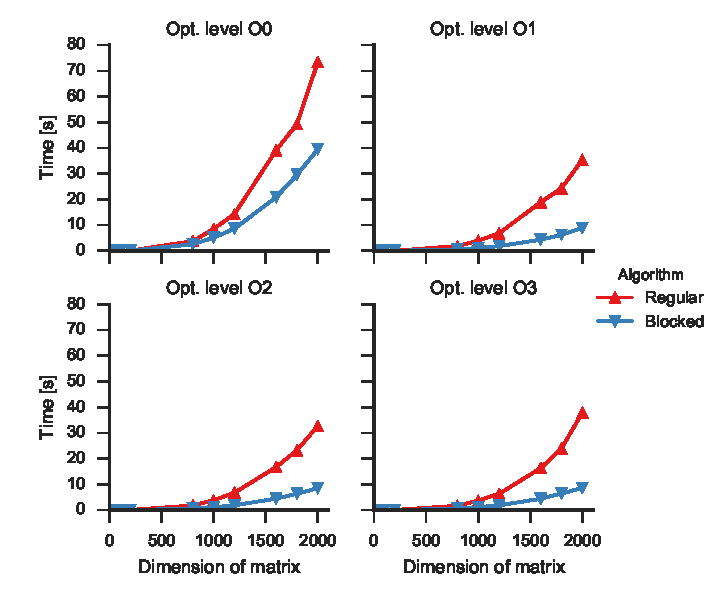
\includegraphics{opttime.pdf}} \\
    \subfloat[Compared across optimization levels]{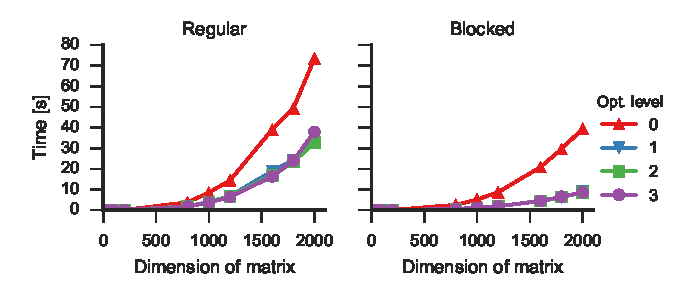
\includegraphics{algotime.pdf}\hspace{1cm}}
    \caption{The timing results, shown in two ways.}
    \label{fig:times}
\end{figure}

\begin{figure}[p]
    \centering
    \subfloat[Compared across algorithms]{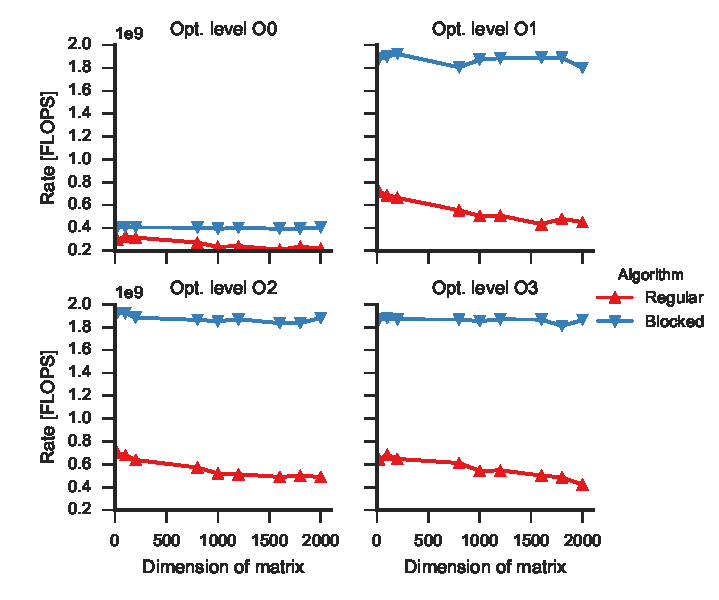
\includegraphics{optrate.pdf}} \\
    \subfloat[Compared across optimization levels]{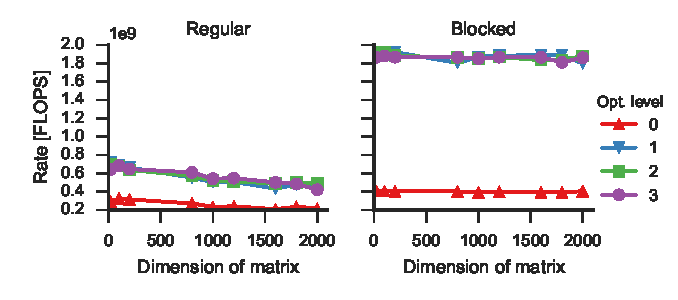
\includegraphics{algorate.pdf}\hspace{1cm}}
    \caption{The rate results, shown in two ways.}
    \label{fig:rates}
\end{figure}

\end{document}
